% id: 119-79
% book: 100발100중 3-2 중간 · 01 3-2 중간(삼각비·삼각비의 활용·원과 직선·원주각·부록)
% section: 족집게 마무리 객관식 80선
% figure: crop:fig-119-79.png
% answer: ③
% answer_source: 답지(빠른정답)
% variant_level: 0 (원본 전사)
% 이 파일은 build.mjs 가 items.json 에서 만든다. 고칠 때는 items.json 을 고친다.
\smash{\raisebox{1.5mm}{\dmkichul{100발100중 3-2 중간 119쪽 79번}}}
\noindent\begin{minipage}[t]{0.58\linewidth}\vspace{0pt}\raggedright 그림에서 원~$\pt{O}$는 $\triangle\pt{ABC}$의 외접원이다. $\arc{AB}:\arc{BC}:\arc{CA}=5:6:7$일 때, $\angle\pt{BAC}$의 크기는?\end{minipage}\hfill\begin{minipage}[t]{0.4\linewidth}\vspace{0pt}\centering 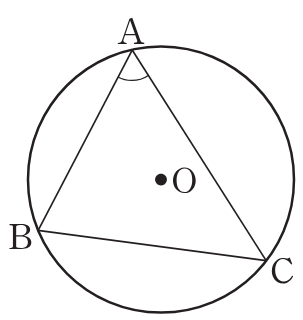
\includegraphics[width=72.5pt]{figures/fig-119-79.png}\end{minipage}\par
\begin{choicesii}{$40^\circ$}{$50^\circ$}{$60^\circ$}{$70^\circ$}{$80^\circ$}\end{choicesii}
